\section{Evaluation}
\label{sec:eval}
In this section we measure prefetch download times and discuss strategies for providing scalability.  We also
look at the transaction manager and evaluate conflict resolution times.

% \begin{figure}[htb!]
% \begin{center}
% 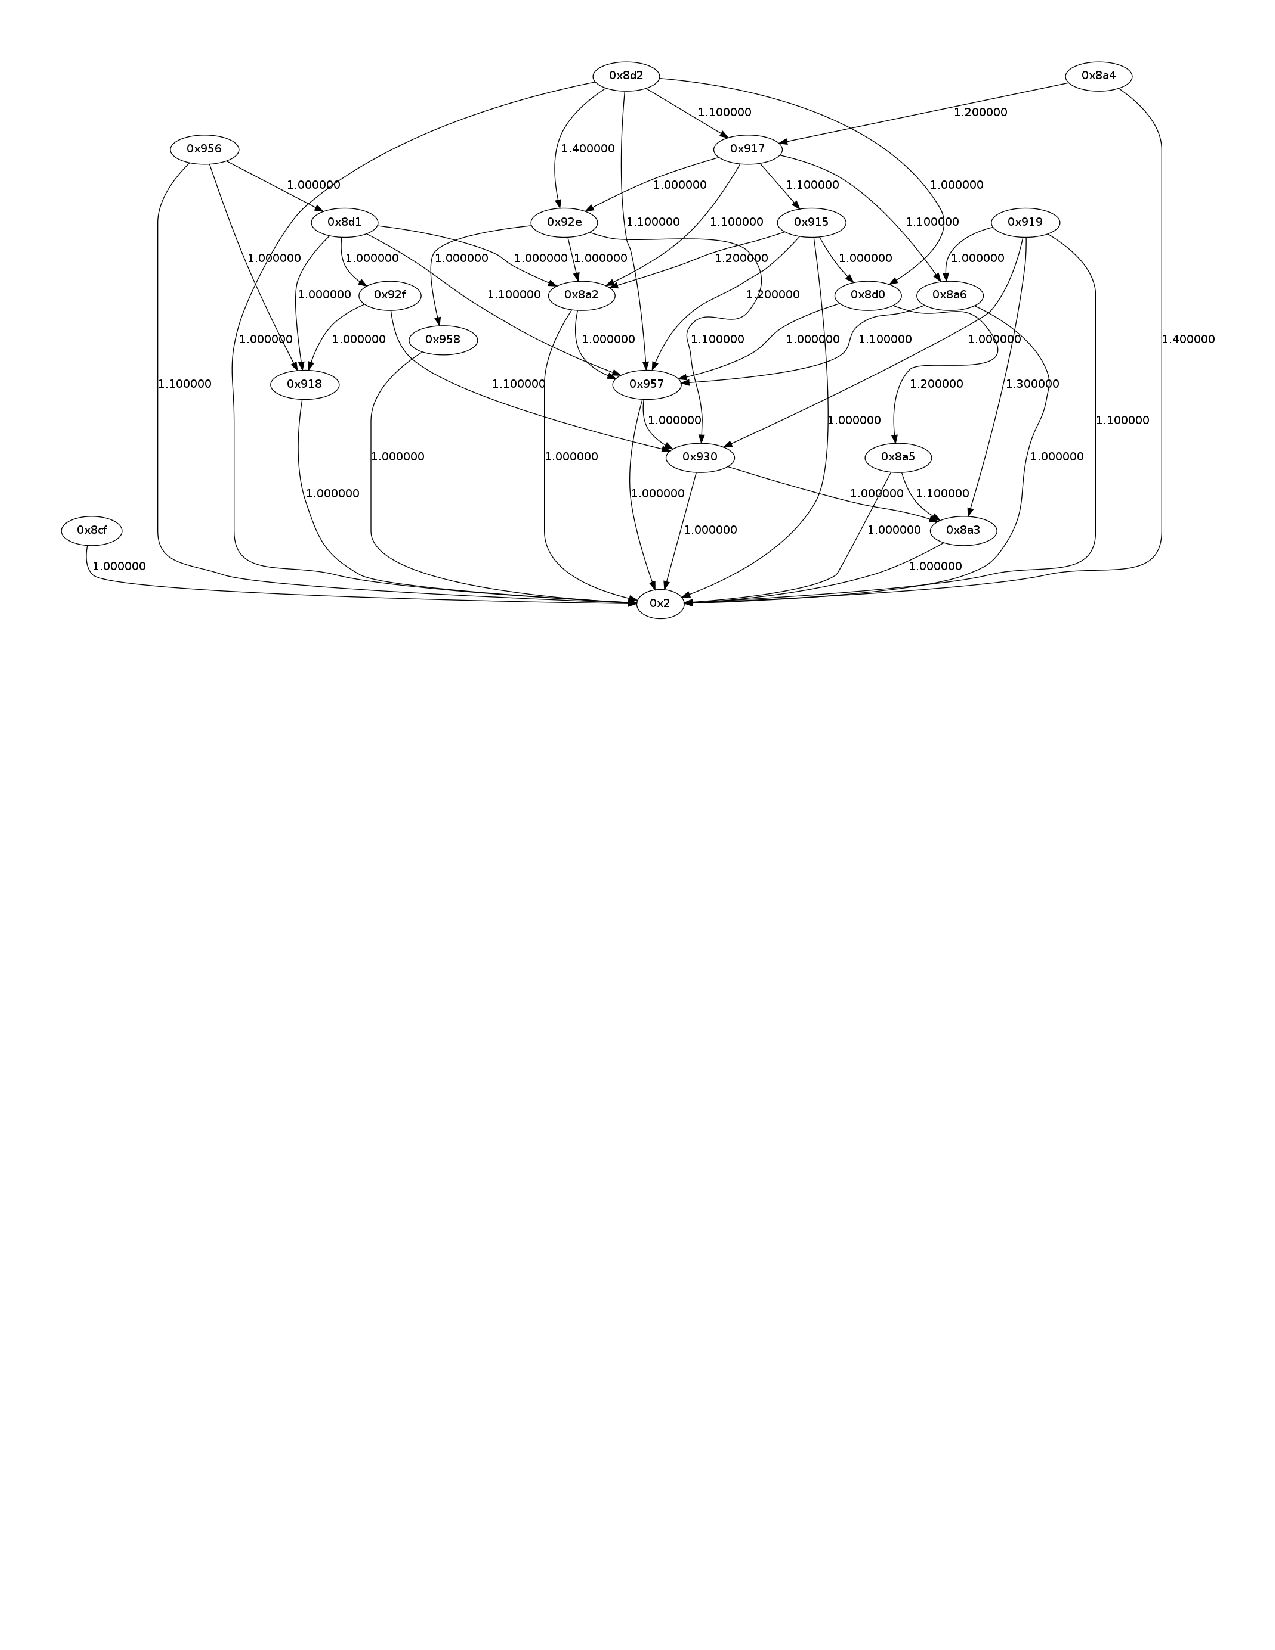
\includegraphics[scale=0.4]{figs/acmenetwork_SDH_4F}
% \caption{}
% \label{fig:acmenetwork_SDH_4F}
% \end{center}
% \end{figure}


\subsection{Prefetching}
Prefetching occurs when a user enters a new floors, as detected by a floor scan or an item
scan.  Table~\ref{tab:prefetchtimes} shows that the prefetch times scale linearly with the number of
items (and data) to prefetch.  Each node holds approximate 100 bytes or information and for
a 20-node deployment of power meters, producing 100 bytes of data per stream (3) every 20 seconds, we fetch 
approximately 1 MB of data.

These prefetch times are non-trivial to deal with, especially since they cause the phone application to slow down
until the data received and loaded into the local cache.  The overhead is dominated by the query in StreamFS that 
constructs the entire sub graph to send to the application.  For future work,  we are will implement a
callback facility and pass the application a reference to it.  The app can then periodically check back until
the query completes and the data is ready to be downloaded.  We can also include partial responses to the query
in the prefetch loop response.  This also allows user to continue using the application without any frustrating waits.

% \subsection{Log dump measurements}
\begin{table}
\begin{center}
  \begin{tabular}{| r | c  c | }
    \hline
    {\bf No. nodes } & {\bf Fetch time (sec) } & {\bf Std. Error (sec)} \\ \hline
    1 & 0.8902 & 0.0756 \\ \hline
    10 & 5.7342 & 1.7087 \\ \hline
    100 & 52.3145 & 14.1146 \\ 
    \hline
  \end{tabular}
\caption{Shows the time to fetch nodes based on the size of the fetch.  The fetch time
increased linearly with the number of nodes.  Caching maintain fetch time near
that of fetching a single node.  A callback is used when cache is invalidated.}
\label{tab:prefetchtimes}
\end{center}
\end{table}


\subsection{Log replay latency}
Table~\ref{tab:optimes} shows the  operation that the transaction manager calls on the StreamFS server.
Log replay and transaction processing is entirely dependent on the time to execute these operations on StreamFS.
There are two types of transactions, a \emph{move}, a \emph{un/bind}, \emph{un/attach}.  A move is a combination
of a `delete' and a `create link', a bind is a `create link' and an `update tags', an unbind and unattach is a
`delete' and `undate tag'.  The transaction latency is the sum of these operations.  By far the most expensive
operation is a `create node' operation.  This occurs when a user adds a new item/space/person to the graph.
The time to apply the operation scale linearly with the size of the logs.  

All logs dumps are processed sequentially.  However, for future work we look to parallelize processing into
parallel processes updating different portions of the graph.  For example, log updates rooted at different floors
could occur simultaneously.




% The global transaction manager implements three main high-level operations -- rollback, apply, and replay.  Our current implementation
% is limited by the time is takes to perform an operation on StreamFS.  Table~\ref{tab:optimes} shows the three 
% main operation that the transaction manager needs to do on the server.
% % Maybe we include another table that talks about the trace we ran through and the conflict times, etc.

% Usually rollbacks consist of \emph{delete} operation and applies consist of \emph{creates}.  In a worst-cases analysis
% of performance we expect the total conflict resolution time to be roughly bounded by
% $rollback\_time + apply\_time + replay\_time$, since $replay\_time=3 X rollback\_time$ and apply\_time is negligible, 
% the total time is approximately $4 X rollback\_time$.  Therefore the overhead is driven by how many new links were created
% that have to be deleted and then re-created.  As an optimization, we limit the scope of a rollback.  The naive
% approach is to blindly undo all operations up to a certain time.  However, we can use the location of the node
% in the ERG to limit the conflict-scope to a sub graph, rather than the entire graph.  The simplest approach is to check if the operation
% on a node either shares an immediate parent with the node that will have an operation undone on it or it the operation
% is on the same node.  By limiting conflict-scope we minimize the number of operation that get execute and, hence, minimize the 
% cost of resolution.



\begin{table}
\begin{center}
  \begin{tabular}{| l | c  c | }
    \hline
    {\bf Operation } & {\bf Avg. exec. time (ms) } &\\ \hline
    fetch & 250 &\\ \hline
    delete & 326  &\\ \hline
    update tags & 267  &\\ \hline
    create link & 250  &\\ \hline
    create node & 1036  &\\ 
    \hline
  \end{tabular}
\caption{Average operation execution time in StreamFS.}
\label{tab:optimes}
\end{center}
\end{table}

% \begin{itemize}
% \item Forwarding
% \item Conflict resolution
% \end{itemize}




% The main driver for the EnergyLens work is to explore the fundamental challenges related to:

% \begin{enumerate}
% \item Tracking people and objects.
% 	\begin{itemize}
% 	\item Through local crowd-sourcing of the tasks to building occupants
% 	\end{itemize}
% \item Maintaining consistency between the relationship between physical items and the entity-relationship graph that represents it.
% \item Providing real-time statistics, information, and processing of energy data related to the building environment.

% 	\begin{itemize}
% 	\item With respect to the occupants
% 	\item with respect to spaces
% 	\item Maintaining security and privacy
% 		\begin{itemize}
% 		\item specifically with respect to personal data and control
% 		\end{itemize}
% 	\end{itemize}

% \end{enumerate}

